\documentclass[journal]{../../IEEEtran/IEEEtran}

\usepackage[activeacute, spanish]{babel} % p/idioma espaniol
\usepackage[utf8]{inputenc}
\usepackage[T1]{fontenc}
\usepackage{cite}



% *** GRAPHICS RELATED PACKAGES ***
%
\ifCLASSINFOpdf
\usepackage[pdftex]{graphicx}
\usepackage{float}
  % declare the path(s) where your graphic files are
  % \graphicspath{{../pdf/}{../jpeg/}}
  % and their extensions so you won't have to specify these with
  % every instance of \includegraphics
  % \DeclareGraphicsExtensions{.pdf,.jpeg,.png}
\else
  % or other class option (dvipsone, dvipdf, if not using dvips). graphicx
  % will default to the driver specified in the system graphics.cfg if no
  % driver is specified.
  % \usepackage[dvips]{graphicx}
  % declare the path(s) where your graphic files are
  % \graphicspath{{../eps/}}
  % and their extensions so you won't have to specify these with
  % every instance of \includegraphics
  % \DeclareGraphicsExtensions{.eps}
\fi


% *** MATH PACKAGES ***
%
%\usepackage{amsmath}
% A popular package from the American Mathematical Society that provides
% many useful and powerful commands for dealing with mathematics.
%
% Note that the amsmath package sets \interdisplaylinepenalty to 10000
% thus preventing page breaks from occurring within multiline equations. Use:
%\interdisplaylinepenalty=2500
% after loading amsmath to restore such page breaks as IEEEtran.cls normally
% does. amsmath.sty is already installed on most LaTeX systems. The latest
% version and documentation can be obtained at:
% http://www.ctan.org/pkg/amsmath


% *** SPECIALIZED LIST PACKAGES ***
%
%\usepackage{algorithmic}
% algorithmic.sty was written by Peter Williams and Rogerio Brito.
% This package provides an algorithmic environment fo describing algorithms.
% You can use the algorithmic environment in-text or within a figure
% environment to provide for a floating algorithm. Do NOT use the algorithm
% floating environment provided by algorithm.sty (by the same authors) or
% algorithm2e.sty (by Christophe Fiorio) as the IEEE does not use dedicated
% algorithm float types and packages that provide these will not provide
% correct IEEE style captions. The latest version and documentation of
% algorithmic.sty can be obtained at:
% http://www.ctan.org/pkg/algorithms
% Also of interest may be the (relatively newer and more customizable)
% algorithmicx.sty package by Szasz Janos:
% http://www.ctan.org/pkg/algorithmicx



% *** PDF, URL AND HYPERLINK PACKAGES ***
%
\usepackage{url}
% url.sty was written by Donald Arseneau. It provides better support for
% handling and breaking URLs. url.sty is already installed on most LaTeX
% systems. The latest version and documentation can be obtained at:
% http://www.ctan.org/pkg/url
% Basically, \url{my_url_here}.

\usepackage{hyperref}


% *** Do not adjust lengths that control margins, column widths, etc. ***
% *** Do not use packages that alter fonts (such as pslatex).         ***
% There should be no need to do such things with IEEEtran.cls V1.6 and later.


% correct bad hyphenation here
\hyphenation{op-tical net-works semi-conduc-tor}


\begin{document}
\title{Calculadora graficadora}


\author { W.~E.~S.~Tubín \thanks{W.~E.~S.~Tubín actualmente
    estudia en Ingeniería en Ciencias y Sistemas de la Universidad de
    San Carlos de Guatemala. } }


% The paper headers
\markboth{Universidad de San Carlos, Mayo~2018. \LaTeX\  }%
{Shell \MakeLowercase{\textit{et al.}}: Bare Demo of IEEEtran.cls for IEEE Journals}

\maketitle

% As a general rule, do not put math, special symbols or citations
% in the abstract or keywords.
\begin{abstract}
  Se documenta la realización de una calculadora graficadora,
  utilizando el lenguaje de bajo nivel ensamblador. El programa que
  ensambla es NASM. La ejecución se realizó haciendo una emulación en
  DOSBox.
\end{abstract}


\begin{IEEEkeywords}
Consola, DOSBox, Ensamblador, NASM.
\end{IEEEkeywords}



% For peer review papers, you can put extra information on the cover
% page as needed:
% \ifCLASSOPTIONpeerreview
% \begin{center} \bfseries EDICS Category: 3-BBND \end{center}
% \fi
%
% For peerreview papers, this IEEEtran command inserts a page break and
% creates the second title. It will be ignored for other modes.
% \IEEEpeerreviewmaketitle



\section{Introducción}
% The very first letter is a 2 line initial drop letter followed
% by the rest of the first word in caps.
% 
% form to use if the first word consists of a single letter:
% \IEEEPARstart{A}{demo} file is ....
% 
% form to use if you need the single drop letter followed by
% normal text (unknown if ever used by the IEEE):
% \IEEEPARstart{A}{}demo file is ....
% 
% Some journals put the first two words in caps:
% \IEEEPARstart{T}{his demo} file is ....
% 
% Here we have the typical use of a "T" for an initial drop letter
% and "HIS" in caps to complete the first word.
\IEEEPARstart{L}{a} aplicación consiste en una calculadora que permite
ingresar una función polinómica de hasta grado 4, cuyas operaciones
son: derivar, integrar y graficar. También resolver ecuaciones de
grado no mayor a dos. Las raíces que puede encontrar son enteras
signadas (positivas y negativas). Dichas funciones pueden ser
ingresadas manualmente y mediante un archivo de entrada.

La implementación se realiza en ensamblador utilizando NASM version
2.13.03. Se utilizan solo instrucciones para CPU 8086 para DOS. Para
probar el ejecutable se emplea DOSBox.

La interracción con el usuario se logra empleando interrupciones.

Para la graficación se emplea el modo de video 13h.

Se utiliza 16 bits para representar un número signado. Esto quiere
decir que las cantidades que puede manejar están entre $-(2^{16}-1)/2$
y $+(2^{16}-1)/2$.

Los términos \textit{función} y \textit{polinomio} se toman como
sinónimos.

\section{Funcionalidades}
Estas son la opciones del menú principal:

\begin{enumerate}
\item Derivar función: Se ingresa una función de grado máximo 4 de
  coeficientes enteros signados y de dos digitos como máximo. La misma
  se ingresa mediante una cadena e inmediatamente se calcula la
  \textit{derivada} de la función ingresada. Se guarda en memoria
  tanto la función ingresada como la derivada calculada.
\item Integrar función: Se ingresa una función de grado máximo 4 de
  coeficientes enteros signados y de dos digitos como máximo. La misma
  se ingresa mediante una cadena e inmediatamente se calcula la
  \textit{integral} de la función ingresada. Se guarda en memoria
  tanto la función ingresada como la integral calculada.
\item Ingresar funciones: se escribe la ruta del archivo y se deriva,
  integra o resuelven las funciones contenidas en él. Se guarda en
  memoria cada funcion así como su derivada, integral o soluciones.
\item Imprimir funciones ingresadas: Se listan las funciones en el
  sistema así como su derivada, integral o soluciones dependiendo de
  que operación se haya elejido durante su ingreso.
\item Graficar: Se grafican las funciones del sistema. Esto incluye
  los polinomios (las originales) y sus derivadas e integrales.
\item Resolver ecuación: Se ingresa una ecuación de grado no mayor a
  dos y se calcula su(s) solucion(es).
\item Reportes: Muestra un menú en el que es posible crear reportes
  para las funciones del sistema a las cuales se calcularon sus
  derivadas o integrales o bien a los que se les encontró sus
  raices. Para el primer caso también se muestran cinco puntos
  evaluados en la función.
\item Salir: Sale del programa.
\end{enumerate}

Observaciones:
\begin{itemize}
\item El \textit{máximo numero de funciones} posibles en el sistema es
  de quince. Al llegar a este número muestra un mensaje que los
  espacios se han llenado.
\item Cada que se ingresa una funcion, vía archivo o manualmente, se
  realiza un \textit{análisis léxico} de la cadena ingresada para
  validarla. En caso de que sea una cadena errónea se muestran los
  mensajes pertinentes.
\end{itemize} 

\section{Autómata}
La validación para la cadena de entrada del polinomio, tanto manual
como mediante archivo, se logra realizando un análisis
lexico. Simultáneamente conforme va validado va cargando en memoria
los coeficientes y exponentes si todo es correcto. Si se llega a un
'';'' y no ocurrio error se aumenta el contador global de funciones
del sistema que puede encontrarse en el archivo \verb|anlex2.asm| y
se llama \verb|n_pol|.

La funcion ''scanner'' es la que implementa el autómata realizando el
análisis léxico de una función polinómica de grado 4 con coeficientes
de dos digitos positivos o negativos. Un término correcto debe iniciar
con ''+'' o ''-'' seguido de cero, uno o dos digitos. Luego puede
venir o no una ''x'' o bien ''x'' seguido por ''2'' o ''3'' o
''4''. La expresión regular es la siguiente:
\begin{verbatim}
ER=(('+'|'-')(<d>?<d>)?[x^<expo>|x]?)+;
donde: <d>=0|1|2|3|4|5|6|7|8|9 y <expo>=2|3|4
\end{verbatim}

Estos son algunos ejemplos de cadenas lexicamente correctas para este
lenguaje (debe terminar en '';''):
\begin{verbatim}
+2x+1-99x  +29  +x +29;
-90x^3 +5  5x^2;
\end{verbatim}

  % /*   0      1      2      3      4      5      6      | <-Entrada  */
  % /*   +      -      d      x      ^   EXPONE   FDC     |            */

\begin{table}[H]
  \centering
  \caption{Tabla de transiciones empleada}
  \begin{tabular}{cccccccc}
 Estado/Entrada&         +&     -&     d&     x&     z&   expo&   FDC \\ \hline
      A&         	  B&     B&   -& -& -& -& -\\
B&	-& -&   C&     D&   -& -& -\\
C&	  B&     B&     E&     D&   -& -& \#\\
D&	  B&     B&   -& -&   F&   -& \#\\
E&	  B&     B&   -&   D&   -& -& \#\\
F&	-& -& -& -& -&   D&   -
  \end{tabular}
\end{table}

Las casillas con ''-'' son estados de error y los ''\#'' estados de aceptación.

\begin{figure}[H]
  \centering
  \caption{Diagrama de transiciones}
  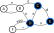
\includegraphics{grafo.pdf}
\end{figure}

No se diagramaron las transiciones desde los estados de aceptación C,
D, y E hacia B, con entradas ''+'' y ''-'' por comodidad visual. De
todas formas puede consultarlo en la tabla de transiciones.

\section{Modo de video utilizado}
Se utilizó \textbf{Int 10/AH=00/AL=13H}. Esta es una interrupción que
establece el modo de video \cite{int10_00_13}. Recibe \verb|00h| en
\verb|AH| y el modo de video en \verb|AL|, que en este caso es
\verb|13h|.

Este modo de video es modo grafico 40x25 de 256 colores, 320x200
pixeles y 1 página. Salidas:

\begin{itemize}
\item AL = bandera de modo de video
  \begin{itemize}
  \item 20h modo > 7
  \item 30h modos 0-5 y 7
  \item 3Fh modo 6
  \end{itemize}
\item AL = CRT byte del modo controlador.
\end{itemize}

\section{Interrupciones}
Estas son las interrupciones utilizadas.

\subsection{Int 10h}

\subsubsection{AH=02h}
Es una interrupción de video y establece la posición del
cursor\cite{int10_02h}. En BH va el número de página. En DH va la fila
(00h es arriba). En DL va la columna (en 00h es izquierda). Salidas:
\begin{itemize}
\item Nada
\end{itemize}

\subsubsection{AH=06h}
Es una interrupción de video y desplaza la ventana hacia
arriba\cite{int10_06h}. En AL recibe número de líneas para desplazarse
hacia arriba (00h = borrar toda la ventana). En BH el atributo
utilizado para escribir líneas en blanco en la parte inferior de la
ventana. En CH y CL la fila y columna de la esquina superior izquierda
de la ventana. En DH y DL la fila y columna de la esquina inferior
derecha de la ventana. Salidas:
\begin{itemize}
\item Nada
\end{itemize}


\subsubsection{AH=0Fh}
Es una interrupción de video y obtiene el modo de video
actual\cite{Int10_0Fh}. Salidas:
\begin{itemize}
\item AH = número de columnas de caracteres
\item AL = modo de visualización
\item BH = página activa .
\end{itemize}



\subsection{Int 21h}

\subsubsection{AH=4Ch}
Es una interrupción de DOS. Termina con código de
retorno\cite{int21_4c}. En \verb|AH| recibe \verb|4ch|. En \verb|AL|
recibe el código de retorno. Salidas:
\begin{itemize}
\item Nada.
\end{itemize}

\subsubsection{AH=0Ah}
Lee una cadena de caracteres desde el dispositivo de entrada estándar
hasta que se presiona la tecla Enter (cuando se detecta retorno de
carro). Comprueba para Ctrl-Break y Ctrl-C \cite{int21_0ah}. En DS:DX
va el puntero al buffer de entrada. Este buffer debe tener un formato
determinado que se muestra a continuación:


\begin{table}[H]
  \centering
  \caption{Formato de DOS para el buffer de entrada \cite{int21_0ah_tabla}}
  \begin{tabular}{llp{5.5cm}}
    \hline
    Offset & Size & Descripcion\\
    \hline
    00h & BYTE & caracteres maximo que el buffer puede manejar\\
    01h & BYTE & numero de caracteres leído, excluyendo retorno de carro\\
    02h & n BYTES & puntero al primer caracter de la cadena leída. Esta cadena incluye el retorno de carro\\
    \hline
  \end{tabular}
\end{table}

El \textit{Offset} se refiere al desplazamiento a partir del puntero
inicial. Por ejemplo cuando se indica offset de 00h, en realidad se
trata del primer byte del arreglo, si así lo queremos ver. Salidas:
\begin{itemize}
\item Buffer lleno con la entrada del usuario.
\end{itemize}


\subsection{Int 1A}

\subsubsection{AH=00h}
Es una interrupción de tiempo y obtiene el tiempo del sistema
\cite{int1a_00}. Salidas:
\begin{itemize}
\item CX:DX =número de ciclos por segundo desde la media noche.
\item AL=bandera de medianoche, distinta de cero si ha pasado la
  medianoche desde la última vez que se leyó.
\end{itemize}


\subsection{Int 16}

\subsubsection{AH = 01h}
Es una interrupción de teclado y comprueba si hay pulsación de teclado
en el buffer.  \cite{int16_01}. Salidas:
\begin{itemize}
\item Establece ZF si no hay pulsación de teclado disponible
\item Resetea ZF si hay pulsación de teclado disponible
\item AH = Código de BIOS escaneado
\item AL = Caracter ASCII
\end{itemize}


\subsubsection{AH = 00h}
Es una interrupción de teclado y obtiene la pulsación de teclado
del buffer sin eco.  \cite{int16_00}. Salidas:
\begin{itemize}
\item AH = Código de BIOS escaneado
\item AL = Caracter ASCII
\end{itemize}

\subsection{Int 15}

\subsubsection{AH = 86h}
Es una interrupción del BIOS espera los microsegundos indicados en
\verb|CX:DX| \cite{int15_86}. Salidas: 
\begin{itemize}
\item resetea CF si fue exitoso (intervalo de espera transcurrido)
\item establece CF en caso de error o AH=83h espera ya en progreso
\item AH =  estado
\end{itemize}

\section{Archivo io.mac}
\label{sec-1}
Macros para entrada y salida utilizando interrupciones. Son
ejecutables en DOS. Para emular DOS se utilizó DOSBox. Es ensamblado
por NASM.
  
\subsection{TERMINAR\_PROGRAMA}
\label{sec-1-1}
Salir del programa
\begin{itemize}
\item Entrada
\begin{description}
\item[vacio] nada
\end{description}
\item Salida
\begin{description}
\item[vacio] nada
\end{description}
\end{itemize}

\subsection{PRINT}
\label{sec-1-2}
Imprimir cadena en salida estandar.
\begin{itemize}
\item Entrada
\begin{description}
\item[dx,\%1] puntero a cadena que termina en ''\$''
\end{description}
\item Salida
\begin{description}
\item[vacio] nada
\end{description}
\end{itemize}

\subsection{PRINT\_CHAR}
\label{sec-1-3}
Imprimir caracter en la salida estandar
\begin{itemize}
\item Entrada
\begin{description}
\item[dl,\%1] el caracter a imprimir
\end{description}
\item Salida
\begin{description}
\item[al] la ultima salida de caracter
\end{description}
\end{itemize}
\href{http://www.ctyme.com/intr/rb-2554.htm}{ir}

\subsection{ABRIR\_ARCHIVO}
\label{sec-1-4}
Abre un archivo existente.
\begin{itemize}
\item Entrada
\begin{description}
\item[dx,\%1] puntero a cadena con nombre/ruta del archivo a
abrir. Este nombre debe finalizar en 0
\end{description}
\item Salidas
\begin{description}
\item[CF=0] archivo se abrio exitosamente. En AX el handle
del archivo
\item[CF=1] ocurrio algun error. El código del error en AX
\end{description}
\end{itemize}
\href{http://www.ctyme.com/intr/rb-2779.htm}{ir}

\subsection{LEER\_ARCHIVO}
\label{sec-1-5}
Lee archivo abierto.
\begin{itemize}
\item Entradas
\begin{description}
\item[bx,\%1] handle del archivo
\item[cx,\%2] numero de bytes a leer
\item[dx,\%3] buffer en donde guardar lo leido
\end{description}
\item Salidas
\begin{description}
\item[CF=0] se leyo exitosamente. En AX el numero de bytes
actualmente leídos
\item[CF=1] ocurrio algun error. El código del error en AX
\end{description}
\end{itemize}
\href{http://www.ctyme.com/intr/rb-2783.htm}{ir}


\subsection{ESENAR}
\label{sec-1-6}
EScribir EN un ARchivo abierto
\begin{itemize}
\item Entradas
\begin{description}
\item[bx,\%1] handle del archivo
\item[cx,\%2] numero de bytes a escribir
\item[dx,\%3] puntero a array que se escribirá
\end{description}
\item Salidas
\begin{description}
\item[CF=0] se escribió exitosamente. En AX el numero de
bytes actualmente escritos.
\item[CF=1] ocurrio algun error. El código del error en AX
(05h,06h).
\end{description}
\end{itemize}
\href{http://www.ctyme.com/intr/rb-2791.htm}{ir}


\subsection{CERRAR\_ARCHIVO}
\label{sec-1-7}
Cierra un archivo
\begin{itemize}
\item Entrada
\begin{description}
\item[bx,\%1] handle del archivo a cerrar
\end{description}
\item Salida
\begin{description}
\item[CF=0] se cerro exitosamente. AX destruido
\item[CF=1] ocurrio algun error al cerrar. En AX el código
de error (06h).
\end{description}
\end{itemize}

\subsection{CREAR\_ARCHIVO}
\label{sec-1-8}
Crear un archivo nuevo o truncar si ya existe.
\begin{itemize}
\item Entrada
\begin{description}
\item[dx,\%1] puntero a cadena que será nombre del
archivo. Este nombre debe terminar en 0.
\end{description}
\item Salida
\begin{description}
\item[CF=0] se creo exitosamente. En AX el handle de
archivo.
\item[CF=1] ocurrio algun error al crear En AX el código
de error (03h,04h,05h).
\end{description}
\end{itemize}
\href{http://www.ctyme.com/intr/rb-2778.htm#Table1401}{ir}


\subsection{UBICAR\_CURSOR}
\label{sec-1-9}
ubicar cursor en la pantalla cuando se esta en modo
texto.
\begin{itemize}
\item Entradas
\begin{description}
\item[dh,\%1] fila
\item[dl,\%2] columna
\end{description}
\end{itemize}


\subsection{LIMPIAR\_PANTALLA}
\label{sec-1-10}
Limpiar pantalla cuando se esta en modo texto.
\begin{itemize}
\item Entrada
\begin{description}
\item[vacio] nada
\end{description}
\item Salida
\begin{description}
\item[vacio] nada
\end{description}
\end{itemize}


\subsection{DESPLAZAR\_ARRIBA}
\label{sec-1-11}
Desplaza hacia arriba. Es como borrar la pantalla según los
parámentros explicados a  continuación:
\begin{itemize}
\item Entrada
\begin{description}
\item[ch,\%1] fila superior izquierda
\item[cl,\%2] columna superior izquierda
\item[dh,\%3] fila inferior derecha
\item[dl,\%4] columna inferior derecha
\item[al,\%5] número de líneas a desplazarse hacia arriba
\end{description}
\item Salida
\begin{description}
\item[vacio] nada
\end{description}
\end{itemize}

\href{http://www.ctyme.com/intr/rb-0096.htm}{ir}


\subsection{GETCHAR}
\label{sec-1-12}
Obtiene ascii de tecla presionada sin eco, via BIOS.
\begin{itemize}
\item Entrada
\begin{description}
\item[vacio] nada
\end{description}
\item Salida
\begin{description}
\item[AL] en este registro se almacena el caracter leido
\end{description}
\end{itemize}

\subsection{READ\_FOR\_BUFF\_INPUT}
\label{sec-1-13}
lee cadena de entrada estandar y lo guarda un arreglo. Se
refirá a este arreglo como buffInput, de aqui en adelante. 
\begin{itemize}
\item Entradas
\begin{description}
\item[dh,\%1] fila
\item[bx,\%2] columna
\item[dx,\%3] arreglo donde guardar la entrada del usuario
\end{description}
\item Salida
\begin{itemize}
\item arreglo buffInput con la entrada del usuario. La
interrupcion utilizada deja dicho arreglo en el
siguiente formato, suponiedo que el usuario ingreso
la cadena ''cad'' en la entrada estandar:
\begin{verbatim}
+--+---+---+---+---+----+---+
|41| 3 | c | a | d | \r |.. |
+--+---+---+---+---+----+---+
\end{verbatim}

donde:
\begin{itemize}
\item\relax [buffInput] contiene 41, indica el numero maximo de
chars que puede guardar
\item\relax [buffInput+1] contiene 3 indica el numero de chars
ingresados por el usuario
\item\relax [buffInput+2] contiene ''c'' es el primer char de la
cadena ingresada. La siguientes dos posiciones tiene
''a'' y ''d''
\item\relax [buffInput+5] contiene el retorno de carro. El
contenido del resto del arreglo esta indefinido
\end{itemize}
\end{itemize}
\end{itemize}

\subsection{READ\_FOR\_BUFF\_INPUT}
\label{sec-1-14}
Lee cadena de entrada estandar y lo guarda un arreglo. NO
necesita de fila y columna.
\begin{itemize}
\item Entradas
\begin{description}
\item[dx,\%1] arreglo donde guardar la entrada del usuario
\end{description}
\item Salida
\begin{itemize}
\item arreglo buffInput con la entrada del usuario.
\end{itemize}
\end{itemize}

\subsection{PRINT}
\label{sec-1-15}
Imprimir cadena en salida estandar en una fila y columna
especificada.
\begin{itemize}
\item Entrada
\begin{description}
\item[dh,\%1] fila
\item[dl,\%2] columna
\item[dx,\%3] puntero a cadena que termina en ''\$''
\end{description}
\item Salida
\begin{description}
\item[vacio] nada
\end{description}
\end{itemize}

\subsection{GETCHAR}
\label{sec-1-16}
Obtiene ascii de tecla presionada, aunque se emplea para
parar el programa, hasta que el usuario presione alguna
tecla, mostrando un mensaje que venga al caso.
\begin{itemize}
\item Entrada
\begin{description}
\item[\%1] Puntero a cadena que se mostrara.
\end{description}
\item Salida
\begin{description}
\item[AL] en este registro se almacena el caracter leido
\end{description}
\end{itemize}

\section{Archivo anlex2.asm}
\label{sec-2}
Contiene la funcion ''scanner'' que realiza el analisis lexico de una
funcion polinomica de grado 4 con coeficientes de dos digitos
positivos o negativos. Un termino correcto debe iniciar con ''+'' o ''-''
seguido de cero, uno o dos digitos. Luego puede venir o no una ''x'' o
bien ''x'' seguido por ''2'' o ''3'' o ''4''. La expresion regular es la
siguiente:
\begin{verbatim}
ER=(('+'|'-')(<d>?<d>)?[x^<expo>|x]?)+;
donde: <d>=0|1|2|3|4|5|6|7|8|9 y <expo>=2|3|4
\end{verbatim}

Estos son algunos ejemplos de cadenas lexicamente correctas para este
lenguaje (debe terminar en '';''):
\begin{verbatim}
+2x+1-99x  +29  +x +29;
-90x^3 +5  5x^2;
\end{verbatim}


\subsection{scanner}
\label{sec-2-1}

Realiza un analisis lexico de la cadena terminada en '';''. Muestra fila
y columna si ocurre error. Muestra exito si se reconoce la
cadena. Guarda los exponentes y coeficientes en una arreglo de
estructuras.

\begin{itemize}
\item Parametro
\begin{description}
\item[[BP+6]] puntero al primer elemento del arreglo de chars a
analizar
\item[[BP+4]] puntero a estructura que guarda coeficientes y
exponentes y otros datos de la funcion.
\end{description}
\item Variables Locales
\begin{enumerate}
\item\relax [BP-2]  fila
\item\relax [BP-4]  columna
\item\relax [BP-6]  entrada
\item\relax [BP-8]  estado
\item\relax [BP-0xA]  exponente
\item\relax [BP-0xC]  primer char ascii de un coeficiente
\item\relax [BP-0xE]  segundo char ascii de un coeficiente
\item\relax [BP-0x10]  tercer char ascii de un coeficiente
\item\relax [BP-0x12]  numero de chars que forman el coeficiente
\item\relax [BP-0x14] contador de terminos por funcion
\end{enumerate}
\end{itemize}


\subsection{scanner\_f}
\label{sec-2-2}
Lo mismo que scanner solo que trabaja con un archivo.

\begin{itemize}
\item Parametro
\begin{description}
\item[[BP+6]] handle del archivo de donde lee
\item[[BP+4]] puntero a estructura que guarda coeficientes y
exponentes y otros datos de la funcion.
\end{description}
\item Variables Locales
\begin{enumerate}
\item\relax [BP-2]  fila
\item\relax [BP-4]  columna
\item\relax [BP-6]  entrada
\item\relax [BP-8]  estado
\item\relax [BP-0xA]  exponente
\item\relax [BP-0xC]  primer char ascii de un coeficiente
\item\relax [BP-0xE]  segundo char ascii de un coeficiente
\item\relax [BP-0x10]  tercer char ascii de un coeficiente
\item\relax [BP-0x12]  numero de chars que forman el coeficiente
\item\relax [BP-0x14] contador de terminos por función
\end{enumerate}
\end{itemize}

\subsection{rutinaDeError}
\label{sec-2-3}
Imprime un mensaje de error lexico.
\begin{itemize}
\item Parametros
\begin{description}
\item[[bp+8]] Fila en binario
\item[[bp+6]] Columna en binario
\item[[bp+4]] El caracter ascii que causo el error
\end{description}
\item Entrada
\begin{description}
\item[bx] puntero a cadena que describe el error
\end{description}
\item Salidas
\begin{description}
\item[vacio] nada
\end{description}
\end{itemize}

\subsection{convNumStrParaNumBin}
\label{sec-2-4}
Convertir numero en string a numero en binario para el manejo interno
como cantidad de la representacion numerica de la cadena. Se utilizó
para leer la cadena directamente de la pila.

\begin{itemize}
\item Entradas
\begin{description}
\item[di] puntero al primer elemento del arreglo de caracteres
(cadena) a convertir. Cada caracter debe estar a cada dos
bytes. Esto es porque se utilizó para leer de la pila cuyos
elementos son de 2 bytes.

\item[cl] tamaño de la cadena apuntada por bx
\end{description}

\item Salida
\begin{description}
\item[ax] el numero de 1 word en binario. En complemento a dos si es
negativo.
\end{description}

\item Variable local
\begin{description}
\item[[BP-2]] variable temporal (temp) que guarda la cantidad que
finalmente se guarda en ax al terminar el proceso
\end{description}
\end{itemize}

\subsection{convNumStrParaNumBin\_arr}
\label{sec-2-5}
Igual que ''convNumStrParaNumBin'' solo que el array de caracteres deben
estar a cada byte no a cada dos, esto para que no necesariamente deba
leerse desde la pila.
\begin{itemize}
\item Entradas
\begin{description}
\item[di] puntero al primer elemento del arreglo de caracteres
(cadena) a convertir.
\item[cl] tamaño de la cadena apuntada por di
\end{description}

\item Salida
\begin{description}
\item[ax] el numero de 1 word en binario. En complemento a dos si es
negativo.
\end{description}

\item Variable local
\begin{description}
\item[[BP-2]] variable temporal (temp) que guarda la cantidad que
finalmente se guarda en ax al terminar el proceso
\end{description}
\end{itemize}

\subsection{printNumBin}
\label{sec-2-6}
Imprimir numero binario en la salida estandar
\begin{itemize}
\item Entradas
\begin{description}
\item[ax] el numero binario (word) a imprimir
\end{description}
\item Salidas
\begin{description}
\item[vacio] nada
\end{description}
\end{itemize}


\subsection{printNumBin\_mas}
\label{sec-2-7}
Lo mismo que printNumBin solo que los positivos les antepone el signo
positivo ''+''
\begin{itemize}
\item Entradas
\begin{description}
\item[ax] el numero binario (word) a imprimir
\end{description}
\item Salidas
\begin{description}
\item[vacio] nada
\end{description}
\end{itemize}


\section{Archivo ploter.asm}
\label{sec-3}

\subsection{dibujar\_plano}
\label{sec-3-1}
dibuja los ejes X y Y del plano cartesiano
\begin{itemize}
\item Parámetros
\begin{description}
\item[[BP+6]] posición x del origen
\item[[BP+4]] posición y del origen
\end{description}
\end{itemize}

\subsection{putPixel}
\label{sec-3-2}
Pinta un pixel en cordenada y color dado. Las coordenadas
son con respecto al origen del plano establecido durante la
llamada ha ''dibujar\_plano''.
\begin{itemize}
\item Entradas
\begin{description}
\item[dl] color
\item[bx] coordenada x
\item[ax] coordenada y
\end{description}
\end{itemize}

\subsection{dibujar\_linea\_horizontal}
\label{sec-3-3}
dibuja una linea horizontal
\begin{itemize}
\item Parámetros
\begin{description}
\item[[BP+10]] color
\item[[BP+8]] ancho
\item[[BP+6]] x
\item[[BP+4]] y
\end{description}
\end{itemize}


\subsection{dibujar\_linea\_vertical}
\label{sec-3-4}
Dibuja una linea vertical
\begin{itemize}
\item Parámetros
\begin{description}
\item[[BP+10]] color
\item[[BP+8]] alto
\item[[BP+6]] x
\item[[BP+4]] y
\end{description}
\end{itemize}

\subsection{dibujar\_rectangulo}
\label{sec-3-5}
Dibuja un rectangulo relleno de un color dado.
\begin{itemize}
\item Parámetros
\begin{description}
\item[[BP+12]] color
\item[[BP+10]] ancho
\item[[BP+8]] alto
\item[[BP+6]] x
\item[[BP+4]] y
\end{description}
\end{itemize}

\section{Archivo rep.asm}
\label{sec-4}
\subsection{printPol\_f}
\label{sec-4-1}
Imprimir polinomio en archivo
\begin{itemize}
\item Parametros
\begin{description}
\item[[BP+6]] handle del archivo
\item[[BP+4]] puntero al inicio del arreglo que contiene la
expresion polinomica
\end{description}
\end{itemize}

\subsection{printCoef\_f}
\label{sec-4-2}
Imprimir coeficiente en archivo
\begin{itemize}
\item Parametros
\begin{description}
\item[[PB+8]] handle del archivo
\item[[BP+6]] coeficiente en binario (word)
\item[[BP+4]] exponente en binario (byte)
\end{description}
\end{itemize}

\subsection{printNumBin\_f}
\label{sec-4-3}
Imprimir numero binario en archivo
\begin{itemize}
\item Parametro
\begin{description}
\item[[BP+6]] valor para saber si se quiere imprimir los
positivos anteponiendo un ''+''. Si tiene el
valor de POS\_CON\_MAS se imprime el ''+''
\item[[BP+4]] handle del archivo
\end{description}
\item Entradas
\begin{description}
\item[ax] el numero binario (word) a imprimir
\end{description}
\item Variables locales
\begin{description}
\item[[BP-2]] un temporal para ax
\item[[BP-4]] un temporal para bx
\item[[BP-6]] un temporal para cx
\end{description}
\end{itemize}

\section{Archivo calgra.asm}
\label{sec-5}

\subsection{evalPol}
\label{sec-5-1}
Evaluar polinomio de 5 terminos como maximo
\begin{itemize}
\item Entradas:
\begin{description}
\item[di] puntero a estructura que contiene el
polinomio a evaluar
\end{description}
\item Parámetros
\begin{description}
\item[[PB+4]] número a evaluar de un word (x)
\end{description}
\item Variables locales
\begin{description}
\item[[BP-2]] temporal que al final será ax
\item[[BP-4]] contador para bucle mayor
\end{description}
\item Salidas
\begin{description}
\item[ax] el resultado de la evaluación (y)
\end{description}
\end{itemize}


\subsection{printInfoEsquina}
\label{sec-5-2}
imprimir cantidad de polinomios actuales en el sistema y
cuanto es el maximo que puede ingresarse. Esto en la
esquina inferior derecha.


Crear reportes.
\begin{itemize}
\item Variables locales
\begin{description}
\item[[BP-2]] handle de archivo ya sea el creado para
polinomios del sistema o bien el creado para
ecuaciones resueltas. Es uno o el otro nunca
ámbos.
\item[[BP-4]] contador del bucle
\item[[BP-6]] para llevar la letra de cada funcion
\item[[BP-8]] temporal para la evaluacion de puntos
\item[[BP-10]] igual que el anterior
\end{description}
\end{itemize}

\subsection{setOrientacionPol}
\label{sec-5-3}
Establecer si un polinomio de grado 1,2,3 o 4, es positivo
o negativo. Para uso exclusivo de rutina \texttt{conocerGrado}.
\begin{itemize}
\item Entradas
\begin{description}
\item[bx] coeficiente del termino de exponenete mayor
\end{description}
\item Salidas
\begin{description}
\item[ah] POL\_POSITIVO si positivo y POL\_POSITIVO-1 si
negativo
\end{description}
\end{itemize}


\subsection{conocerGrado}
\label{sec-5-4}
Saber el grado de un polinomio
\begin{itemize}
\item Entradas
\begin{description}
\item[di] puntero a estructura que contiene el polinomio
\end{description}
\item Salidas
\begin{description}
\item[al] grado del polinomio
\item[ah] POL\_POSITIVO si positivo y POL\_POSITIVO-1 si
negativo
\end{description}
\end{itemize}


\subsection{Graficar polinomios}
\label{sec-5-5}
\begin{itemize}
\item Variables locales
\begin{description}
\item[[bp-2]] contador temporal para bucle mayor
\item[[bp-4]] limite inferior del rango a graficar (x0)
\item[[bp-6]] limite superior del rango a graficar (x1)
\item[[bp-8]] factor por el cual se dividen los puntos en
el eje Y, dependiendo si se trata de un
polinomio de 1,2,3 o 4 grado, esto para que
se logre la visualización más adecuada de la
gráfica considerando que se tiene solo 200
pixeles del modo de video para el eje Y.
\end{description}
\end{itemize}


\subsection{printIntegral}
\label{sec-5-6}
Imprime una integral en salida estandar. Basicamente es lo
mismo que printPol, la diferencia es que antes de hacer la
llamada a printPol imprime la notacion de integrales.
\begin{itemize}
\item Entrada
\begin{description}
\item[si] polinomio integrado
\end{description}
\end{itemize}


\subsection{printDerivada}
\label{sec-5-7}
Imprime una derivada en salida estandar. Basicamente es lo
mismo que printPol, la diferencia es que antes de hacer la
llamada a printPol imprime la notacion de derivadas.
\begin{itemize}
\item Entrada
\begin{description}
\item[si] polinomio derivado de otro polinomio
\end{description}
\end{itemize}


\subsection{printPolinomio}
\label{sec-5-8}
Imprime una integral en salida estandar. Basicamente es lo
mismo que printPol, la diferencia es que antes de hacer la
llamada a printPol imprime la notacion de funcion
identificandola con una letra mayuscula.
\begin{itemize}
\item Entrada
\begin{description}
\item[di] polinomio original que no es derivada ni integral
de otro polinomio
\end{description}
\end{itemize}


\subsection{printCoef}
\label{sec-5-9}
Imprimir coeficiente en la salida estandar
\begin{itemize}
\item Parametros
\begin{description}
\item[[BP+6]] coeficiente en binario (word)
\item[[BP+4]] exponente en binario (byte)
\end{description}
\end{itemize}

\subsection{printPol}
\label{sec-5-10}
Imprimir polinomio en salida estandar
\begin{itemize}
\item Parametros
\begin{description}
\item[[BP+4]] puntero al inicio del arreglo que contiene la
expresion polinomica
\end{description}
\end{itemize}

\subsection{integrarPol}
\label{sec-5-11}
Integra una polinomio de 5 terminos como maximo
\begin{itemize}
\item Entrada:
\begin{description}
\item[di] puntero a estructura que contiene el polinomio a
integrar.
\item[si] puntero a estructura donde guardar la integración.
\end{description}
\end{itemize}

\subsection{integrarPol}
\label{sec-5-12}
Integra una polinomio de 5 terminos como maximo
\begin{itemize}
\item Entrada:
\begin{description}
\item[di] puntero a estructura que contiene el polinomio a
derivar.
\item[si] puntero a estructura donde guardar la derivación.
\end{description}
\end{itemize}


\subsection{ing}
\label{sec-5-13}
Opcion ''ingresar'' del menú principal, cuyo objetivo es
cargar un archivo con expresiones polinómicas terminadas en
'';''
\begin{itemize}
\item Variables Locales
\begin{description}
\item[[BP-2]] guarda el handle del archivo abierto.
\end{description}
\end{itemize}


%%% Local Variables:
%%% mode: latex
%%% TeX-master: "tec"
%%% End:


\section{Conclusión}
El lenguaje ensamblador es de bajo nivel y ayuda a compreder mejor el
funcionamiento de los registros y memoria de una computadora. Así
mismo DOS escribir un programa en ensamblador, para DOSBox ayuda a
tener una mejor panorámica sobre las bases de sistemas operativos mas
actuales como MS-Widonws.


% if have a single appendix:
%\appendix[Proof of the Zonklar Equations]
% or
%\appendix  % for no appendix heading
% do not use \section anymore after \appendix, only \section*
% is possibly needed

% use appendices with more than one appendix
% then use \section to start each appendix
% you must declare a \section before using any
% \subsection or using \label (\appendices by itself
% starts a section numbered zero.)
%



% \appendices
% \section{Secuencia para controlar motores paso a paso bipolares}


% use section* for acknowledgment
% \section*{Acknowledgment}


% The authors would like to thank...


% Can use something like this to put references on a page
% by themselves when using endfloat and the captionsoff option.
\ifCLASSOPTIONcaptionsoff
  \newpage
\fi

% trigger a \newpage just before the given reference
% number - used to balance the columns on the last page
% adjust value as needed - may need to be readjusted if
% the document is modified later
%\IEEEtriggeratref{8}
% The "triggered" command can be changed if desired:
%\IEEEtriggercmd{\enlargethispage{-5in}}

% references section

% can use a bibliography generated by BibTeX as a .bbl file
% BibTeX documentation can be easily obtained at:
% http://mirror.ctan.org/biblio/bibtex/contrib/doc/
% The IEEEtran BibTeX style support page is at:
% http://www.michaelshell.org/tex/ieeetran/bibtex/
%\bibliographystyle{IEEEtran}
% argument is your BibTeX string definitions and bibliography database(s)
%\bibliography{IEEEabrv,../bib/paper}
%
% <OR> manually copy in the resultant .bbl file
% set second argument of \begin to the number of references
% (used to reserve space for the reference number labels box)
\begin{thebibliography}{15}

  % -------------------- INT 10 --------------------  
\bibitem{int10_02h}
  Ralf Brown's. \emph{VIDEO - SET CURSOR POSITION},
  Disponible:
  \urlstyle{tt}\url{http://www.ctyme.com/intr/rb-0087.htm}

\bibitem{int10_06h}
  Ralf Brown's. \emph{VIDEO - SCROLL UP WINDOW},
  Disponible:
  \urlstyle{tt}\url{http://www.ctyme.com/intr/rb-0096.htm}
    
  
\bibitem{Int10_0Fh}
  Ralf Brown's. \emph{VIDEO - GET CURRENT VIDEO MODE},
  Disponible:
  \urlstyle{tt}\url{http://www.ctyme.com/intr/rb-0096.htm}

\bibitem{int10_00_13}
  Ralf Brown's. \emph{VIDEO - SET VIDEO MODE},
  Disponible:
  \urlstyle{tt}\url{http://www.ctyme.com/intr/rb-0069.htm}

\bibitem{int10_ahE}
  Ralf Brown's. \emph{TELETYPE OUTPUT},
  Disponible:
  \urlstyle{tt}\url{http://www.ctyme.com/intr/rb-0106.htm}  

  % -------------------- INT 1A --------------------
\bibitem{int1a_00}
  Ralf Brown's. \emph{TIME - GET SYSTEM TIME},
  Disponible:
  \urlstyle{tt}\url{http://www.ctyme.com/intr/rb-2271.htm}


  % -------------------- INT 15 --------------------
\bibitem{int15_86}
  Ralf Brown's. \emph{BIOS - WAIT (AT,PS)},
  Disponible:
  \urlstyle{tt}\url{http://www.ctyme.com/intr/rb-1525.htm}  
  

  % -------------------- INT 16 --------------------
\bibitem{int16_00}
  Ralf Brown's. \emph{KEYBOARD - GET KEYSTROKE},
  Disponible:
  \urlstyle{tt}\url{http://www.ctyme.com/intr/rb-1754.htm}
  
\bibitem{int16_01}
  Ralf Brown's. \emph{KEYBOARD - CHECK FOR KEYSTROKE},
  Disponible:
  \urlstyle{tt}\url{http://www.ctyme.com/intr/rb-1755.htm}  
  
  % -------------------- INT 21 --------------------
\bibitem{int21_4c}
  Ralf Brown's. \emph{EXIT - TERMINATE WITH RETURN CODE},
  Disponible:
  \urlstyle{tt}\url{http://www.ctyme.com/intr/rb-2974.htm}

\bibitem{int21_0ah}
  Vitaly. \emph{Buffered Input},
  Disponible:
  \urlstyle{tt}\url{http://vitaly_filatov.tripod.com/ng/asm/asm_010.11.html}

\bibitem{int21_0ah_tabla}
  Ralf Brown's. \emph{BUFFERED INPUT},
  Disponible:
  \urlstyle{tt}\url{http://www.ctyme.com/intr/rb-2563.htm#Table1344}
   
  
\bibitem{21h_40h}
  Jones ICS. \emph{File Processing},
  Disponible:
  \urlstyle{tt}\url{http://fleder44.net/312/notes/16Files/Index.html}
  
  % -------------------- OTROS --------------------  
\bibitem{nasm}
  Wikipedia. \emph{Archivos COM},
  Disponible:
  \urlstyle{tt}\url{https://es.wikipedia.org/wiki/Netwide_Assembler}
  
\bibitem{com}
  Wikipedia. \emph{Archivos COM},
  Disponible:
  \urlstyle{tt}\url{https://es.wikipedia.org/wiki/Archivo_COM}
  

  
\end{thebibliography}

% biography section
% 
% If you have an EPS/PDF photo (graphicx package needed) extra braces are
% needed around the contents of the optional argument to biography to prevent
% the LaTeX parser from getting confused when it sees the complicated
% \includegraphics command within an optional argument. (You could create
% your own custom macro containing the \includegraphics command to make things
% simpler here.)
%\begin{IEEEbiography}[{\includegraphics[width=1in,height=1.25in,clip,keepaspectratio]{mshell}}]{Michael Shell}
% or if you just want to reserve a space for a photo:

% \begin{IEEEbiography}{Michael Shell}
% Biography text here.
% \end{IEEEbiography}

% if you will not have a photo at all:
\begin{IEEEbiographynophoto}{W.~E.~S.~Tubín (201213139)}
nació en Guatemala, Guatemala. Estudia ingeniería en Ciencias y
Sistemas en la Universidad de San Carlos de Guatemala.
\end{IEEEbiographynophoto}


% insert where needed to balance the two columns on the last page with
% biographies
%\newpage

% \begin{IEEEbiographynophoto}{Jane Doe}
% Biography text here.
% \end{IEEEbiographynophoto}

% You can push biographies down or up by placing
% a \vfill before or after them. The appropriate
% use of \vfill depends on what kind of text is
% on the last page and whether or not the columns
% are being equalized.

\vfill

% Can be used to pull up biographies so that the bottom of the last one
% is flush with the other column.
%\enlargethispage{-5in}



% that's all folks
\end{document}